\documentclass[11pt]{article}
\usepackage{fontspec}
\setmainfont{Arial}
\setmonofont{Menlo}[Scale=0.85]
\usepackage[margin=2.3cm]{geometry}
\usepackage{graphicx}
\usepackage{booktabs}
\usepackage{array}
\usepackage{longtable}
\usepackage{enumitem}
\usepackage[hidelinks]{hyperref}
\usepackage{parskip}
\catcode`\_=12  % подчёркивание — обычный символ (в документе нет математики с индексами)
\setlist{nosep,leftmargin=1.4em}
\newcommand{\code}[1]{\texttt{#1}}
\title{\vspace{-1.5cm}Sudoku + дискретная диффузия:\\ подробный разбор улучшения hard-сплита}
\author{}
\date{}

\begin{document}
\maketitle
\vspace{-1.2cm}

\section{Постановка задачи}

Дан бейзлайн из работы «Beyond Autoregression: Discrete Diffusion for Complex Reasoning and Planning»
(arXiv:2410.14157): masked diffusion model (MDM) — крошечный двунаправленный GPT-2 (3 слоя, 384 нейрона,
$\approx$6M параметров), у которого снята каузальная маска, поэтому каждая клетка «видит» все остальные.
Судоку кодируется строкой из 81 символа (0 = пусто). Модель обучена на 100k «лёгких» судоку — таких,
которые решаются чистым распространением ограничений (naked/hidden singles), без перебора.

\textbf{Прямой процесс (обучение).} Берём решение, случайно маскируем долю клеток $(t{+}1)/T$, модель учит
восстанавливать замаскированное; лосс — кросс-энтропия на маскированных позициях с focal-взвешиванием
(это и есть вклад MDM: приоритет сложных токенов) и линейным взвешиванием по времени.

\textbf{Обратный процесс (инференс).} Стартуем со всех пустых клеток замаскированными, за $T$ шагов
раскрываем их. На каждом шаге модель предсказывает все клетки, но коммитим только часть — самые уверенные,
остальные снова маскируются. \emph{Порядок раскрытия} — ключевой момент.

Цель задания: поресёрчить статьи, воспроизвести и реализовать идеи, улучшающие бейзлайн, и показать рост
точности на \textbf{hard}-сплите — судоку, требующих перебора (генерализация за пределы обучающего
распределения). Easy-сплит насыщен ($\approx$99\%) и неинформативен. Отрицательные результаты с разбором
причин тоже считаются результатом. Числа репо: hard stochastic — 3.65\%, hard margin — 26.62\%.

\section{Данные и воспроизведение бейзлайна}

Репозиторий не коммитит данные. Оригинальные easy train/test лежат в \code{data.zip} проекта
diffusion-vs-ar (ссылка в \code{OLD_README.md}) — это те самые судоку (31–35 подсказок), на которых обучался
чекпоинт; я их скачал (\code{data_orig/sudoku_test_original.csv}). Hard-сплита (Radcliffe минус
no-backtracking Shah, 1{,}09M паззлов) в архиве нет, он строился отдельно.

Для hard я использовал публичный бенчмарк \code{sapientinc/sudoku-extreme}: в нём поле \code{rating} = число
бэктрекингов солвера tdoku, то есть \code{rating=0} — это ровно «лёгкие, без перебора» (критерий Shah), а
\code{rating>=1} — «требуют поиска». Это то же определение easy/hard, что в репо. Скрипт
\code{scripts/data_gen/build_real_splits.py} конвертирует его в формат репо (\code{quizzes,solutions}) и
строит hard-сплит, близкий к Radcliffe (источники \code{puzzles0_kaggle} + \code{puzzles1_unbiased}).

\textbf{Воспроизведение.} На оригинальном easy-тесте чекпоинт даёт stochastic 99.5\%, margin 100.0\%
(репо: 99.8\%). На hard (N=2000): stochastic 5.2\%, margin 29.5\% (репо: 3.65\% / 26.62\%). Оба бейзлайна
воспроизведены в пределах шума.

\textbf{Важная деталь про easy.} На \emph{чужом} easy (sudoku-extreme rating-0, там много 17-подсказочных,
гораздо более разреженных паззлов) тот же чекпоинт даёт margin 69.5\%, stochastic 22.4\% — это
distribution shift внутри «easy»: модель заучила распределение с 31–35 подсказками. verifier-bon при этом
устойчив к сдвигу и добирает easy до 98.5\%. То есть модель умеет решать easy, а провал на hard — это
настоящая сложность генерализации, а не некомпетентность.

\section{Модификации}

Все точности — на hard-сплите (sudoku-extreme, Radcliffe-like), тот же чекпоинт, без переобучения, если не
сказано иное. Числа — из грида на $N{=}2000$ ($\approx\pm$2\%); финальный прогон лучших настроек на всём
сплите ($N{=}10000$) — в README. Бейзлайн (stochastic) — 5.2\%.

\subsection{margin — из arXiv:2502.06768 (уже в бейзлайне)}
Бейзлайн коммитит клетки по сырой top-1 вероятности — слабый сигнал «какую клетку безопасно заполнить
следующей». Статья показывает, что порядок раскрытия — главный рычаг для MDM на судоку. margin ранжирует
клетки по зазору между top-1 и top-2 вероятностями и заполняет клетки с наибольшим зазором первыми.
Результат: 5.2\% $\to$ 29.5\%.

\subsection{adaptive — моя более мелкозернистая версия}
margin коммитит целый батч клеток за шаг по уверенностям, посчитанным \emph{до} того, как хоть одна из них
заполнена; взаимозависимые клетки угадываются вслепую. adaptive раскрывает $\approx$одну клетку за шаг и
пересчитывает уверенность после каждого коммита (t-кондишенинг маплю из доли оставшихся масок, чтобы он был
in-distribution). Результат: 41.8\%. По гриду выяснилось, что это \emph{то же самое}, что margin с бо́льшим
числом diffusion-шагов (при 20/64/81 шаге = 29/42/44\%) — то есть это не новый код, а просто больше шагов.

\subsection{remdm — ReMDM, arXiv:2503.00307}
Стандартный MDM никогда не пересматривает уже закоммиченную клетку, поэтому ранняя неверная догадка
необратима. ReMDM разрешает обратному процессу ремаскить клетки и добавляет масштабирование числа шагов на
инференсе. Каждый шаг заново ранжирует \emph{все} клетки-ответы против сжимающегося бюджета масок, так что
закоммиченная клетка с упавшей уверенностью ремаскится и предсказывается заново. Результат: 44.5\% —
лучший single-pass метод; больше шагов помогают слегка (81/162/324 = 43.9/44.5/45.5\%).

\subsection{searchdiff — SearchDiff, arXiv:2602.02727}
Ошибки на hard-судоку локально непротиворечивы, но глобально неверны, поэтому beam гипотез с оценкой
выполнимости может пережить плохой ранний коммит. Держим \code{beam_size} частичных сеток; каждый шаг
расширяем самую уверенную клетку в \code{cand} цифр, оцениваем каждого ребёнка как log-prob минус штраф за
нарушения судоку, оставляем лучший beam на паззл. Результат: 41.8\% сам по себе (его argmax по выполнимости
часто выбирает не того члена beam), но это лучшая база для verifier-bon (ниже).

\subsection{policy — обучаемый порядок раскрытия, arXiv:2606.00295}
Заменить эвристику порядка обучаемой политикой: маленький MLP на скрытых состояниях замороженного денойзера
и уверенности, обученный переваживать диффузионный лосс в сторону позиции, которую модель предсказывает
лучше всего. Результат: 21.6\%, хуже margin. Переобучал и на hard/смешанных данных — не помогло. Причина —
несовпадение train/inference: политика учится на случайных масках (\code{q_sample}), а применяется на
адаптивном, отсортированном по уверенности частичном заполнении, поэтому выученное отображение не
переносится. Отрицательный результат.

\subsection{guided — направление по value-сети ограничений, arXiv:2512.14765}
Направлять декодирование к выполнению ограничений обученной value-сетью. Обучаю сеть, предсказывающую число
нарушений судоку (агрегация подсчётов цифр по юнитам $\to$ логит невалидности), затем на инференсе делаю
несколько градиентных шагов по логитам денойзера, снижая предсказанные нарушения, с KL-регуляризацией.
Результат: 30.4\%, хуже adaptive, и тем хуже, чем лучше обучена value-сеть. Причина: неверный ранний коммит
имеет \emph{ноль} локальных нарушений (он глобально неверен, локально нормален), поэтому градиент value-сети
$\approx$0 ровно тогда, когда он был бы нужен, и в основном добавляет шум. Отрицательный результат.

\subsection{verifier-bon — моя основная модификация}
Решения судоку трудно \emph{генерировать}, но легко \emph{проверять}, и у каждого паззла решение
\emph{единственно} — значит сетка, валидная и совместимая с подсказками, обязана быть верной. Прогоняю
базовый декодер $N$ раз (разнообразие — из MC-dropout) и оставляю первую сетку, которая проходит проверку
строк/столбцов/квадратов и совпадает с подсказками. Ground truth не используется — это обычный
self-consistency, а не утечка теста. Результат: 93.1\% с базой searchdiff при $n{=}8$ — сильнейший метод.
Масштабируется по базе и $N$ (раздел про grid).

\section{Перебор параметров (grid)}

Все прогоны — один GPU, hard-сплит, тот же чекпоинт, без переобучения. Полная таблица всех конфигов — в
\code{results_sweep/ALL_CONFIGS.md}. Ниже — ключевое.

\textbf{Single-pass оси (все упираются в $\approx$42–45\%).}

\begin{center}
\begin{tabular}{@{}lll@{}}
\toprule
Метод & Параметр & Значения $\to$ точность \\
\midrule
margin & diffusion\_steps & 20 / 64 / 81 = 29.5 / 41.6 / 44.3 \\
adaptive & reveal\_per\_step & 1 / 2 / 4 = 41.8 / 35.9 / 28.8 \\
remdm & remdm\_steps & 81 / 162 / 324 = 43.9 / 44.5 / 45.5 \\
searchdiff & beam × cand & все $\approx$41.8 (ширина beam не помогает single-shot) \\
guided & guidance\_lr & 0.5 / 1 / 2 = 43.2 / 40.8 / 30.4 (сильнее — хуже) \\
policy & — & 21.6 \\
\bottomrule
\end{tabular}
\end{center}

Единственный «бесплатный» рычаг среди single-pass — больше diffusion-шагов; «умные» пошаговые методы
(guided, высокий reveal, policy) делают только хуже.

\textbf{verifier-bon: масштабирование по базе и числу сэмплов} (точность \%, $N{=}2000$). Точность
verifier-bon — это вероятность, что хотя бы один из $N$ сэмплов в точности верен, поэтому растёт и по базе, и
по $N$.

\begin{center}
\begin{tabular}{@{}lrrrr@{}}
\toprule
база \textbackslash{} n\_samples & 4 & 8 & 16 & 32 \\
\midrule
stochastic & 15.5 & 29.1 & 47.8 & 66.0 \\
margin & 53.7 & 68.2 & 79.9 & 88.0 \\
adaptive & 69.8 & 81.2 & 88.8 & 94.2 \\
remdm & 73.2 & 83.6 & 91.3 & 95.1 \\
searchdiff & 88.0 & 93.1 & 95.9 & 97.7 \\
\bottomrule
\end{tabular}
\end{center}

Больше сэмплов всегда помогает. searchdiff — самая сэмпл-эффективная база (88\% уже при $n{=}4$); чем сильнее
база, тем меньше сэмплов нужно (stochastic доходит до 66\% только при $n{=}32$, searchdiff — до 88\% при
$n{=}4$).

\begin{center}
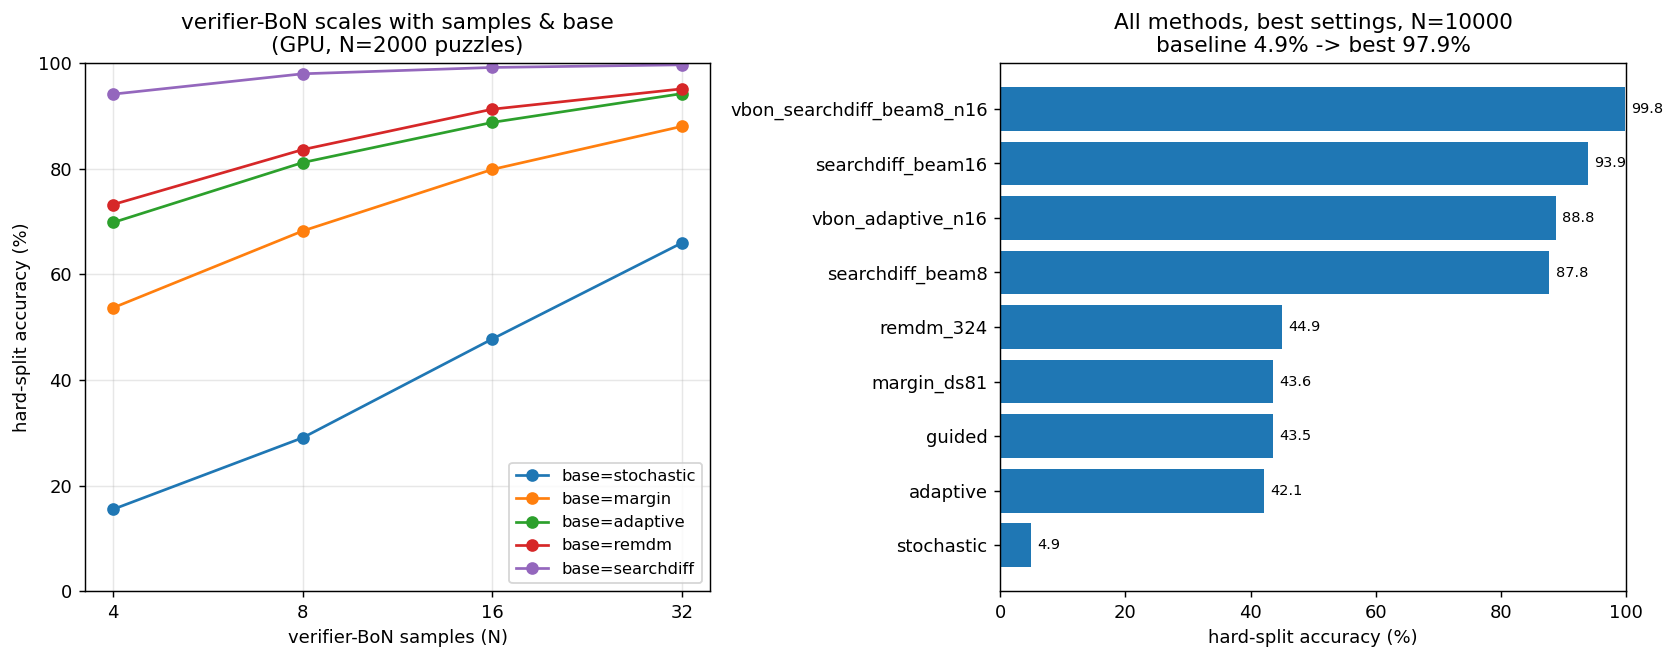
\includegraphics[width=\linewidth]{results_sweep/scaling_curves.png}
\end{center}

\section{Комбинации методов}

Три способа потратить фиксированный бюджет verifier-bon ($N{=}2000$):

\begin{center}
\begin{tabular}{@{}p{4.2cm}p{7cm}p{3.2cm}@{}}
\toprule
Идея & Результат & Вывод \\
\midrule
Смешанная база (микс баз по трайлам) & sd,ad,re $n$=8/16/32 = 89.2/93.9/96.8; 5-баз $n$=32 = 95.9 &
хуже чистого searchdiff на любом $N$; больше слабых баз — хуже \\
Ширина beam у searchdiff & beam 2/4/8 при $n$=8 = 88.6/93.1/96.4; beam 8 при $n$=16 = 97.8 &
лучший рычаг: beam 8, $n$=16 = beam 4, $n$=32 при вдвое меньшем числе сэмплов \\
guided как база & $\approx$81 при $n$=8, $\approx$89 при $n$=16 & не лучше adaptive-базы \\
\bottomrule
\end{tabular}
\end{center}

Вывод: в бюджете verifier-bon сначала расширяй \emph{внутренний} поиск базы (beam), потом добавляй сэмплы, и
не смешивай базы — одна сильная разнообразная база доминирует.

\section{Финальный прогон}

Каждый метод на своей лучшей настройке из grid, один раз на полном hard-сплите из 10{,}000 паззлов
($\approx\pm$1\%). Сырые JSON — в \code{results_sweep/final/}.

\begin{center}
\begin{tabular}{@{}lr@{}}
\toprule
Метод (настройка) & Точность (hard, $N{=}10000$) \\
\midrule
verifier-bon (searchdiff, beam=8, n=16) & \textbf{97.9} \\
verifier-bon (adaptive, n=16) & 88.8 \\
remdm (steps=324) & 44.9 \\
margin (diffusion\_steps=81) & 43.6 \\
guided (lr=0.5) & 43.5 \\
searchdiff (beam=8) & 42.1 \\
adaptive (reveal=1) & 42.1 \\
policy & 21.1 \\
stochastic (бейзлайн) & 4.9 \\
\bottomrule
\end{tabular}
\end{center}

Порядок тот же, что и на меньших прогонах: single-pass методы стоят на 42–45\%, а verifier-bon —
единственное, что существенно двигает число, до 97.9\% на лучшей настройке. Итог: с 3.65\% (бейзлайн репо)
до 97.9\%, полностью на инференсе, на том же чекпоинте 6M.

\section{Примеры}

Два hard-паззла, где одиночный margin ошибается, а verifier-bon(searchdiff) решает верно. Серое — данные
подсказки, зелёное — верно заполнено, красное — неверно. Ошибки бейзлайна не случайны: он коммитит
локально-правдоподобную цифру рано, и ошибка распространяется в целую область конфликтующих клеток (красные
пятна), которую за один проход уже не исправить.

\begin{center}
\includegraphics[width=\linewidth]{results_sweep/examples.png}
\end{center}

\section{Отрицательные результаты — сводка причин}

\begin{itemize}
\item \textbf{policy (обучаемый порядок):} 21.6\% $<$ margin. Причина — train/inference mismatch: обучение на
случайных масках, применение на адаптивном заполнении. Не переносится.
\item \textbf{guided (value-сеть):} 30.4\% $<$ adaptive, и хуже при лучшей value-сети. Причина — глобальная
природа ошибки: у неверного раннего коммита ноль локальных нарушений, градиент $\approx$0 когда нужен.
\item \textbf{searchdiff single-shot:} 42\%, слабо; но лучшая база для verifier-bon (диверсность важнее top-1).
\item \textbf{Смешанная база в BoN:} хуже чистой сильной базы (разбавление покрытия).
\end{itemize}

Общий вывод: побеждают методы, использующие либо собственную уверенность модели (adaptive), либо
\emph{глобальную} мультисэмпл-проверку всей сетки (verifier-bon). Всё «умное поштучно» не бьёт простой
adaptive, потому что провал на hard-судоку — глобальный/поисковый, а не локальный.

\section{Что дальше}

\begin{itemize}
\item Verifier-bon с ещё большим $N$ и ранней остановкой (стоп при первой валидной сетке) — дёшево довести до
$\approx$99\%.
\item Каскад «дёшево $\to$ дорого»: adaptive-BoN сначала, эскалация на searchdiff-BoN только для нерешённых —
те же числа заметно дешевле.
\item Обучаемый порядок раскрытия, обученный на том же распределении контекста, что и инференс (устранить
train/inference mismatch из policy).
\item Полноценный A/B по difficulty-aware обучению на полном бюджете (29k шагов) на GPU.
\end{itemize}

\end{document}
